
\begin{figure*}[th]
\centering
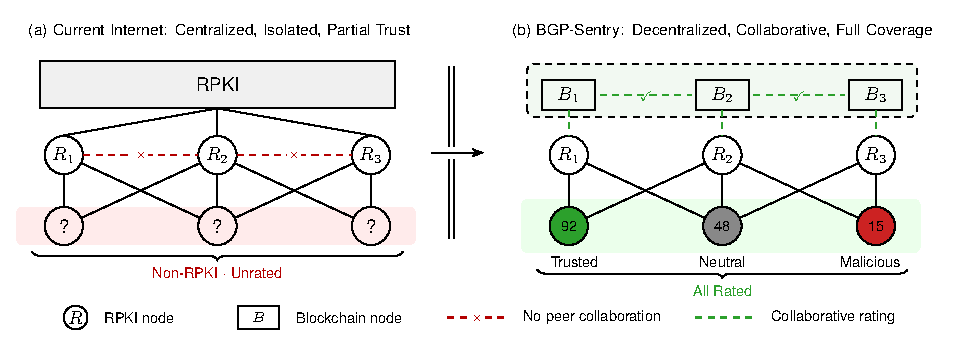
\includegraphics[width=0.85\textwidth]{figures/architecture.pdf}
\vspace{-4pt}
\caption{Before and after BGP-Sentry. \textbf{Left:} Current Internet routing with RPKI-only validation. RPKI-enabled ASes (green, marked ``R'') provide binary VALID/INVALID decisions, but the ${\sim}$63\% of ASes without RPKI (hatched ``?'' nodes) remain completely unverifiable, a blind spot exploitable by attackers. \textbf{Right:} The same network topology after BGP-Sentry deployment. RPKI-enabled ASes serve as behavioral observers (green dotted lines), and every non-RPKI AS receives a graduated trust score: Highly Trusted ($\geq$90, dark blue) through Malicious ($<$30, dark red). The topology, peering relationships, and RPKI/non-RPKI ratio are identical; only the visibility changes. The vertical bar (far right) maps node colors to the five-tier trust classification.}
\label{fig:system-architecture}
\end{figure*}


\section{Expanding BGP Trust via Blockchain Audit Trails}
\label{sec:system_threat_model}
In this section, we present the system and threat model, followed by an overview of BGP-Sentry.

% BGP-Sentry is fundamentally anchored by the \textbf{Central RPKI Infrastructure}~\cite{}, which serves as the system's primary root of trust. Rather than attempting to ``invent'' trust in a decentralized vacuum, we leverage the existing cryptographic certainty of Route Origin Authorizations (ROAs) to provide an authoritative baseline for routing legitimacy. 

\subsection{System Model}
\label{subsec:system_model}

\md{We define the system model for BGP-Sentry over the global inter-domain routing graph $G = (\mathcal{V}, \mathcal{E})$, where $\mathcal{V}$ is the set of Autonomous Systems ($\mathcal{AS}$). Our model builds on the partial deployment of RPKI as its foundation. We designate the subset of RPKI-compliant nodes $\mathcal{O} \subset \mathcal{V}$ as observers. These nodes leverage the global RPKI hierarchy as a root of trust, using cryptographically signed ROAs to verify prefix ownership. These observers also act as a bridge between the legacy BGP environment and our Blockchain security layer; they monitor updates from non-participating neighbors and execute a local detection pipeline to generate evidence for a distributed ledger $\mathcal{L}$. To maintain the integrity of this ledger, we assume a synchronous honest majority within the observer set $\mathcal{O}$, where at least a quorum $\tau$ of the observers involved in a validation task are non-adversarial and maintain consistent RPKI caches. 
Finally, observers leverage existing registries (e.g., RPKI repositories) of participating nodes to identify RPKI peers along a routing path as distributed witnesses for cross-verification before recording data in the immutable audit trail $\mathcal{L}$.}


% For the network data plane, we consider a decentralized BGP monitoring environment consisting of a set of Autonomous Systems $\mathcal{AS}$. 
% The system architecture, BGP-Sentry, is composed of the following components:

% \begin{itemize}

% \item \textbf{Central RPKI (Root of Trust).}
% At the core of our model sits the global RPKI hierarchy. This infrastructure provides the "ground truth" for IP prefix ownership. In our system, every routing observation is measured against this central authority; this ensures that security claims are not merely local opinions but are cryptographically linked to established RPKI credentials.
%     \item \textbf{Distributed RPKI Observers ($\mathcal{O} \subset \mathcal{AS}$).} These are RPKI-enabled nodes that monitor BGP updates from neighboring non-RPKI ASes. They execute the four-detector pipeline (Algorithm~\ref{alg:create_transaction}) and act as validators in the consensus process.
%     \item \textbf{Trust Expansion via RPKI-certified Blockchain ($\mathcal{L}$).} A tamper-evident distributed ledger that stores the global state of AS trust scores, verified attack observations, and the history of prefix announcements.
   
% \end{itemize}

% \BfPara{Realistic Assumptions}
% Our model is grounded in three realistic assumptions that reflect the practice of current BGP infrastructure. First, we do not assume the entire Internet to align overnight~\cite{}, and the system is built for \textit{partial deployment}, requiring only a strategic subset of RPKI-compliant nodes to serve as observers. Within this pool, we rely on a standard \textit{honest majority}~\cite{}, specifically, that at least a quorum $\tau$ of queried observers are non-adversarial and maintain synchronized RPKI caches. Finally, we assume these observers are not flying blind~\cite{}. They must be able to locate one another through the \textit{AS-path discovery} logic we detail in Algorithm~\ref{alg:observer_discovery}, which provides the connectivity needed for effective cross-verification.

\subsection{Threat Model}
\label{subsec:threat_model}
\md{We assume a Byzantine adversary~\cite{lamport2019byzantine} $\mathcal{A}$ representing a malicious or misconfigured Autonomous System (AS), including both non-RPKI participants and potentially compromised nodes within the observer set $\mathcal{O}$. We assume $\mathcal{A}$ is capable of injecting fraudulent routing information, such as prefix/sub-prefix hijacks~\cite{prefixHijacking} and bogon announcements~\cite{mao2003bgp}, to enable traffic interception, Man-in-the-Middle (MitM) attacks, blackholing, or persistent network instability~\cite{butler2009survey}. We assume RPKI compliance does not inherently guarantee benign behavior; thus, $\mathcal{A}$ may reside within $\mathcal{O}$, attempting to disrupt consensus via false observations or collusion to fork the ledger $\mathcal{L}$. However, $\mathcal{A}$ remains computationally bounded and cannot compromise standard cryptographic primitives (e.g., SHA-256), the RPKI root of trust, or the honest majority quorum $\tau$ established in our system model.}


% We define an adversary $\mathcal{A}$ as a malicious or misconfigured non-RPKI Autonomous System. $\mathcal{A}$ can inject fraudulent routing information, specifically: (i) \texttt{PREFIX\_HIJACK}~\cite{}, (ii) \texttt{SUBPREFIX\_HIJACK}~\cite{}, and (iii) \texttt{BOGON\_INJECTION}~\cite{}. $\mathcal{A}$ may also engage in recidivism, launching repeated attacks across different consensus rounds. The primary objectives of $\mathcal{A}$ are traffic interception, Man-in-the-Middle (MitM) attacks \cite{}, or causing network instability. We assume the underlying cryptographic primitives (SHA-256) and the RPKI database itself are secure against direct compromise \cite{}.


\subsection{Overview of BGP-Sentry}
\label{subsec:defense_concept}

We designed BGP-Sentry as a closed-loop framework that transforms transient BGP updates into long-term, actionable routing policy. As shown in Figure~\ref{fig:system-architecture}, while the existing RPKI infrastructure is limited to validating signed prefixes, BGP-Sentry leverages RPKI-compliant nodes as distributed observers to audit the behavior of the broader, non-compliant ASes. The system operates through a continuous four-stage cycle: 

\circled{1} \textbf{Collaborative Observation:} The workflow begins at the network edge, where the RPKI-compliant observers ($\mathcal{O}$) ingest BGP announcements from their peer ASes. Unlike legacy frameworks that generate isolated local alerts, BGP-Sentry leverages these observers as distributed validators. When an observer observes an announcement to detect a potential violation (e.g., prefix hijack), it triggers a global validation request, elevating the event from a local observation to a collective inquiry.

\circled{2} \textbf{Consensus-Based Validation:} To prevent false positives or malicious reporting by a compromised observer, BGP-Sentry employs a Proof-of-Population (PoP) consensus mechanism. The detecting observer coordinates with a quorum $\tau$ of peers identified via the routing path to cross-verify the event. An incident is committed to the ledger once it meets the required consensus threshold. This process ensures that all system announcements are mathematically verifiable, grounding the network's events in a collective truth rather than separated claims.

\circled{3} \textbf{The Forensic Audit Trail:} Once an event is validated, it is recorded in the immutable ledger $\mathcal{L}$, transforming BGP's ephemeral behavior into a persistent, cryptographically verifiable audit trail. This enables future post-hoc analysis of AS behavior, allowing operators to reconstruct its evolution and detect complex coordinated attacks that are invisible to single-node monitoring.

\circled{4} \textbf{Dynamic Trust and Security Enforcement:} The system closes the loop by translating historical evidence into active defense. BGP-Sentry maintains a Dynamic Trust Score $S$ for every non-RPKI entity, initialized at a neutral baseline and adjusted based on verified behavior recorded in $\mathcal{L}$. When an AS's score falls below a critical threshold $\mathcal{T}$, the ledger propagates a ``Malisous'' state across the consortium. \textcolor{red}{Using this, participating routers then automatically trigger \textit{Trust-Based Filtering}, effectively isolating the attacker by rejecting its announcements at the ingress. This ensures that an AS's past behavior directly dictates its current reachability, creating a self-reinforcing deterrent against persistent routing threats.}



\textcolor{OliveGreen}{[Mehdi] @Anik The assumption about RPKI node behavior and the scoring mechanism is vague: 1) on one hand, we are assuming that RPKI nodes can also behave maliciously (which is possible due to misconfiguration or compromise cases), 2) on the other hand, we are only scoring the non-RPKI, then the question is what happens to the RPKI node in the scoring system?}



% BGP-Sentry is architected as a closed-loop security framework that bridges the gap between transient BGP observations and long-term network policy. Unlike traditional monitoring tools that provide isolated alerts, our approach integrates real-time reactive logic with a persistent forensic ledger to create an automated enforcement cycle.

% \BfPara{Reactive Detection and Consensus}
% The loop begins at the network edge, where RPKI observers ($\mathcal{O}$) ingest BGP announcements and execute a multi-stage detection pipeline. When a routing violation is flagged, the system transitions from local observation to global validation. Through the \textit{Proof-of-Population} (PoP) consensus mechanism, the observer coordinates with peers discovered via AS-path analysis (Algorithm~\ref{alg:observer_discovery}) to verify the event. This distributed validation ensures that penalties are only applied to committed transactions that have reached the consensus threshold ($\tau$).

% \BfPara{Post-Hoc Forensic Analysis}
% By treating the blockchain as a tamper-evident "black box," BGP-Sentry enables retrospective security analysis that survives the ephemeral nature of BGP updates. Using forensic primitives like \texttt{get\_attack\_history()}, operators can reconstruct the behavioral evolution of an AS over time. This historical context, cryptographically endorsed by the observer network, transforms raw routing data into actionable evidence, as summarized in the audit trail (Table~\ref{tab:forensic_audit}), which can be used to justify peering changes or legal abuse reports.

% \BfPara{Post-Hoc Forensic Analysis}
% \anik{Beyond real-time detection, the blockchain ledger $\mathcal{L}$ enables retrospective security analyses which is difficult for any single announcement or single observer. Because every record in $\mathcal{L}$ is cryptographically signed by its detecting observer and endorsed by relevant other neighbor observer, post-hoc findings are independently verifiable by any consortium participant, a property that a centralized log cannot provide. The immutable, multi-observer audit trail supports cross-observer correlation to resolve ambiguous real-time signals such as route flapping, accumulation of independent single-witness observations into high-confidence assessments, detection of coordinated multi-AS attack campaigns through temporal analysis, integrity auditing of RPKI observers via voting-pattern anomalies, and longitudinal behavioral pattern detection including trust score gaming. These capabilities are detailed in Section~\ref{subsec:posthoc_building_blocks}.}

% \BfPara{Collaborative Trust Establishment}
% Rather than treating security as a binary "valid or invalid" state, BGP-Sentry introduces a protocol-embedded module designed to quantify the long-term reliability of non-RPKI entities. This module maintains a dynamic reputation score $S \in [0, 100]$ for every non-RPKI AS, serving as a behavioral proxy where cryptographic certificates are absent. We initialize every such AS with a neutral baseline of $S_{initial} = 50$, reflecting a stance of cautious optimism: we assume a "Neutral" posture until observed behavior dictates otherwise. This scoring mechanism is not a subjective "rating" but a deterministic calculation performed during consensus; it ensures that the collective observations of RPKI-enabled peers are distilled into a single, actionable metric. By embedding this logic directly into the protocol, we ensure that trust is established through a shared social contract, where an AS’s ability to interact with the RPKI-protected core is earned through consistent, legitimate routing behavior.

% \BfPara{The Security Enforcement Loop}
% The system closes the loop by mapping this accumulated behavioral evidence to active network defense. The \textit{Reactive Trust Engine} continuously aggregates consensus-verified penalties and recidivism surcharges to update a global trust score ($S$). When an AS's behavior causes it to cross the threshold into the \texttt{Malicious} tier ($S < 30$), the ledger propagates this state across the consortium. Participating routers then automatically trigger \textit{Trust-Based Filtering}, effectively isolating the attacker by rejecting its announcements at the ingress. This cycle ensures that yesterday's confirmed hijack directly dictates today's routing policy, creating a self-reinforcing deterrent against persistent threats.

% % \subsection{System Overview}
% % BGP-Sentry is a blockchain-based framework that transforms RPKI-enabled ASes into distributed observers for rating non-RPKI Autonomous Systems through behavioral trust assessment. The system addresses the fundamental challenge that 40\% of Internet routing operates without RPKI validation by leveraging the 60\% RPKI-enabled infrastructure as a trusted observation network.

% % The architecture consists of three core components: 

% % \noindent\textbf{(1) RPKI Observer Network.} that monitors and reports non-RPKI routing behavior.

% % \noindent\textbf{(2) Proof of Population Consensus Framework \cite{yin2019hotstuff}.} that processes observations, attack classifications, and penalties atomically. \textcolor{red}{What is this reference [20] for?}

% % \noindent\textbf{(3) Trust Rating and Incentive System.} that maintains behavioral accountability through scoring and rewards. All interactions are designed to be recorded on a permissioned blockchain accessible only to RPKI-enabled participants.

 



% \BfPara{Takeaways} Non-RPKI ASes receive \textit{Trust Scores (0-100)} reflecting their routing behavior quality, affecting their network privileges. These scores remain non-tradable to prevent market manipulation of security assessments. \texttt{RPKI observers} earn \texttt{BGP Coins} as incentives to maintain honest, accurate monitoring of \texttt{non-RPKI neighbors}, with potential future financial value to enhance participation motivation. This dual assessment model extends cryptographic trust to non-participating networks while ensuring observer accountability.

% \BfPara{Design Goal}
% We choose a \emph{permissioned} blockchain over public chains (e.g., Ethereum) because RPKI already provides natural access control, permissioned consensus achieves finality in under 3 seconds (vs.\ minutes for public chains), and all participants are accountable RPKI-enabled ASes.
% The \emph{30-second competition window} balances geographic inclusivity (BGP announcements propagate in 2--5 minutes) against attack-response speed.
% \emph{Time-window synchronization} addresses BGP's asymmetric observation problem: nodes independently verify whether observations fall within agreed timestamp boundaries without waiting for global acknowledgment.
% The \emph{combined reporter/merger role} avoids separating transaction submission from block creation, preserving full observational context (timing, AS-PATH, peer relationship) throughout consensus.
% Trust \emph{penalty values} ($P_{bogon}{=}25$, $P_{prefix}{=}20$, $P_{subprefix}{=}18$, $P_{leak}{=}15$, $P_{flapping}{=}10$) reflect attack severity: 2--3 confirmed attacks drop an AS from Neutral to Suspicious, with escalating penalties for repeat offenders.




% \textcolor{blue}{[RJ] My checkpoint, will revisit after \textbf{@Mehdi}'s major revision of the following sections.}





\section{System Building Blocks}
\label{sec:architecture}

This section details the core components that realize the system model and the threat model defined above. Figure~\ref{fig:system-architecture} illustrates the transformation from RPKI-only binary validation to full behavioral trust coverage.

\subsection{RPKI Node Onboarding and Verification}

Our proposed architecture restricts participation in the blockchain-based observation role to RPKI-verified Autonomous Systems through an onboarding and validation procedure (Figure~\ref{fig:onboarding}). During the onboarding phase, a candidate node proves control of a valid RPKI certificate and associated ROAs, and existing members verify these credentials before voting on admission. Upon acceptance, the node is issued a blockchain identity that is cryptographically tied to the RPKI resources it provided and is allowed to join the peer-to-peer blockchain network. After onboarding, the node operates as a fully trusted participant, taking part in consensus, block production, and governance activities. Because blockchain identity is bound to RPKI identity at the time of onboarding, non-RPKI entities are unable to generate valid protocol messages and therefore cannot join or influence the network during this phase. Importantly, once onboarding is complete, the system does not require continuous RPKI verification, which allows future extensions of the model where the blockchain can operate independently of the RPKI infrastructure.

\begin{figure}[t]
\centering
\resizebox{\columnwidth}{!}{%
\begin{tikzpicture}[
    >={Stealth[length=1mm]},
    pbox/.style={rectangle, draw=black!70, rounded corners=2pt,
                  minimum height=0.4cm, font=\scriptsize\bfseries,
                  align=center, line width=0.5pt, inner sep=3pt},
    msg/.style={->, semithick, black!70},
    msgback/.style={->, semithick, black!70, densely dashed},
    mlabel/.style={font=\scriptsize, fill=white, inner sep=1pt},
    vbox/.style={rectangle, draw=green!50!black, fill=green!5, rounded corners=1pt,
                 font=\scriptsize, align=center, inner sep=3pt, line width=0.3pt},
    cbox/.style={rectangle, draw=blue!50, fill=blue!5, rounded corners=1pt,
                 font=\scriptsize, align=center, inner sep=3pt, line width=0.3pt},
    rbox/.style={rectangle, draw=green!60!black, fill=green!12, rounded corners=1pt,
                 font=\scriptsize, align=center, inner sep=3pt, line width=0.3pt},
]

% === PARTICIPANTS (wider spacing for scriptsize) ===
\node[pbox, fill=gray!15] (cand) at (0, 0) {Candidate AS};
\node[pbox, fill=green!15] (vals) at (4, 0) {RPKI Validators};
\node[pbox, fill=blue!10] (chain) at (8, 0) {Blockchain};

% === LIFELINES ===
\draw[gray!25, line width=0.3pt] (0, -0.3) -- (0, -5.5);
\draw[gray!25, line width=0.3pt] (4, -0.3) -- (4, -5.5);
\draw[gray!25, line width=0.3pt] (8, -0.3) -- (8, -5.5);

% === STEP 1 ===
\draw[msg] (0.05, -0.65) -- node[mlabel, above] {\textbf{1.} RPKI cert + ROAs} (3.95, -0.65);

% === STEP 2 ===
\node[vbox] at (4, -1.1) {\textbf{2.} Verify X.509 chain};

% === STEP 3-4: Challenge-response ===
\draw[msg] (3.95, -1.65) -- node[mlabel, above] {\textbf{3.} ROA key challenge} (0.05, -1.65);
\draw[msg] (0.05, -2.15) -- node[mlabel, above] {\textbf{4.} Signed proof} (3.95, -2.15);
\node[vbox] at (4, -2.65) {Prefix $\leftrightarrow$ ASN validated};

% === SYBIL BARRIER (enclosing steps 2-4, with margin) ===
\draw[densely dashed, red!35, semithick, rounded corners=3pt] (-0.9, -0.84) rectangle (5.6, -2.95);
\node[font=\scriptsize\bfseries, red!40!black, fill=white, inner sep=1pt, anchor=south west] at (-0.85, -2.95) {Sybil barrier};

% === STEP 5 ===
\draw[msg] (4.05, -3.35) -- node[mlabel, above] {\textbf{5.} Admission request} (7.95, -3.35);

% === STEP 6 ===
\draw[msgback] (7.95, -3.85) -- node[mlabel, above] {\textbf{6.} Verify + vote} (4.05, -3.85);
\node[cbox] at (8, -4.3) {Quorum $\tau$?};

% === STEP 7 ===
\draw[msg] (7.95, -4.75) -- node[mlabel, above] {\textbf{7.} Blockchain identity issued} (0.05, -4.75);
\node[rbox] at (0, -5.2) {Full participant};


\end{tikzpicture}
}% end resizebox
\caption{RPKI-verified onboarding protocol (sequence diagram). The candidate AS submits its RPKI certificate chain (step~1). Validators verify the X.509 chain against RIR trust anchors (step~2), then challenge the candidate to prove ROA key ownership (steps~3--4). This cryptographic verification forms the Sybil barrier: without a legitimate RPKI certificate, no entity can pass steps 2--4. Upon successful verification, validators broadcast an admission request to the consortium (step~5), where members independently verify and vote (step~6). If the quorum threshold is met, a blockchain identity cryptographically bound to the candidate's RPKI resources is issued (step~7), and the node joins the P2P network as a full consensus participant.}
\label{fig:onboarding}
\end{figure}

\subsection{Observation-Driven Consensus}
 Unlike conventional blockchains where all participants share a global view of pending transactions from memory-pool, BGP monitoring produces fundamentally asymmetric observations: each RPKI observer sees only the announcements that traverse its own network position, and an AS may announce different routes to different neighbors based on local policy, maintenance, or congestion management. This asymmetry means that a routing event observed by one node may be invisible to others, or may appear differently depending on the observer's topological vantage point. In some cases, an announcement may be witnessed by only a few observers—a scenario that can also arise from sophisticated targeted attacks. Reliable behavioral assessment therefore requires aggregating these partial, potentially conflicting views into a coherent longitudinal record, from which the behavior of an unverified AS can be systematically determined. With this challenge in mind, we design the consensus process as follows.

% Single-column version of PoP consensus workflow figure — horizontal DAG layout
% Use \input{sections/fig_pop_consensus_1col} where needed

\begin{figure}[htbp]
\centering
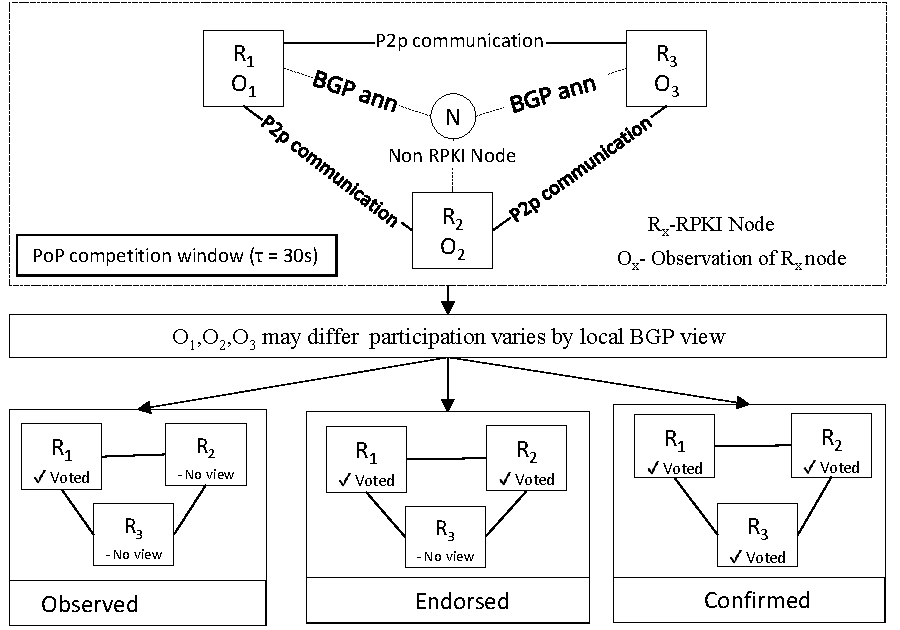
\includegraphics[width=1\columnwidth]{figures/pop.pdf}
 
\vspace{-6pt}
\caption{PoP consensus workflow and blockchain recording. $N$ sends BGP announcements to RPKI observers ($R_1$, $R_2$, $R_3$). Proposer $R_3$ collects peer signatures via P2P and commits the transaction. The zoomed block $B_k$ shows four on-chain data types: the BGP observation, non-RPKI trust score, BGP Coin rewards, and PoP signatures}
\label{fig:pop-consensus-workflow-1col}
\end{figure}



\BfPara{Protocol Design}
In any conventional blockchains, a competition mechanism determines which node will append the next block: Proof-of-Work rewards the fastest computation, while Proof-of-Stake selects validators proportional to locked capital. Both approaches assume a shared transaction pool visible to all participants, reducing consensus to a problem of ordering. On the contrary, BGP-Sentry operates under a fundamentally different premise: because routing observations are asymmetric and no shared mempool exists, the consensus must first establish the validity of an observation before recording it. The competition in our Proof-of-Population mechanism is therefore based on observational corroboration rather than computation or economic stake. When an RPKI observer processes a BGP announcement from a non-RPKI neighbor, it creates a signed transaction and broadcasts a vote request to topologically relevant peers discovered via AS-path analysis (Algorithm~\ref{alg:observer_discovery}). Each peer independently validates the observation against its own local knowledge base, returning an endorsement if it can corroborate the event. The first node to accumulate the required endorsement threshold ($\tau \geq 3$ independent confirmations) commits the transaction to the blockchain. This corroboration-driven design ensures that recorded observations are backed by multiple independent vantage points, while the RPKI-anchored identity system guarantees that each endorsement originates from a distinct, cryptographically verified entity—preventing any single participant from fabricating agreement.


\BfPara{Consensus Protocol Specification}
We formalize the Proof of Population consensus mechanism through four interconnected algorithms. Algorithm~\ref{alg:pop_consensus} presents the main consensus protocol and Algorithm~\ref{alg:create_transaction} specifies atomic transaction creation, both in the main text. The auxiliary algorithms (AS-path observer discovery (Algorithm~\ref{alg:observer_discovery}) and time-bounded vote collection (Algorithm~\ref{alg:signature_collection})) are provided in Appendix~\ref{app:supplementary_algorithms}.

% ============================================
% ALGORITHM 1: MAIN PROOF OF POPULATION CONSENSUS
% ============================================

\begin{algorithm}[t]
\caption{Observation-Driven Consensus Protocol}
\label{alg:pop_consensus}
\begin{algorithmic}[1]
\Statex \textbf{Input:} event $\mathit{e}$, node $\mathit{N_i}$,
\Statex \hspace{2.1em} threshold $\boldsymbol{\tau} = \max(3, \min(\lfloor N/3 \rfloor + 1, 5))$
\Statex \textbf{Output:} transaction $\mathit{TX}$ with consensus status

\Statex \textbf{Step 1: Deduplication}
\State $\mathit{key} \gets (\mathit{prefix}, \mathit{originAS})$
\If{$\mathit{key} \in \mathit{LastSeenCache}$ \textbf{and} $\mathrm{age} < \boldsymbol{T_{\mathrm{sample}}}$}
    \State \Return $\bot$ \Comment{Skip duplicate}
\EndIf

\Statex \textbf{Step 2: Transaction creation and vote collection}
\State $\mathit{TX} \gets \Call{CreateSignedTx}{\mathit{e},\; \mathit{SK_i}}$
\State $\mathit{Obs} \gets \Call{DiscoverObservers}{\mathit{ASpath}}$ \Comment{Alg.~\ref{alg:observer_discovery}}
\State $\Call{BroadcastVoteRequest}{\mathit{TX},\; \mathit{Obs}}$
\State $\mathit{Sigs} \gets \Call{CollectVotes}{\mathit{TX},\; \boldsymbol{\tau},\; \boldsymbol{T_{\mathrm{reg}}}}$ \Comment{Alg.~\ref{alg:signature_collection}}

\Statex \textbf{Step 3: Consensus classification}
\If{$|\mathit{Sigs}| \geq \boldsymbol{\tau}$}
    \State $\mathit{TX}.\mathit{status} \gets$ \texttt{CONFIRMED}
\ElsIf{$|\mathit{Sigs}| \geq 1$}
    \State $\mathit{TX}.\mathit{status} \gets$ \texttt{INSUFFICIENT\_CONSENSUS}
\Else
    \State $\mathit{TX}.\mathit{status} \gets$ \texttt{SINGLE\_WITNESS}
\EndIf

\Statex \textbf{Step 4: Commit and replicate}
\State $\Call{AppendToChain}{\mathit{TX}}$
\State $\Call{ReplicateBlock}{\mathit{TX},\; \mathit{peers}}$
\State \Return $\mathit{TX}$

\end{algorithmic}
\end{algorithm}

% Algorithms 2 (Observer Discovery) and 3 (Vote Collection) are provided in Appendix~\ref{app:supplementary_algorithms}.

% ============================================
% ALGORITHM 4: ATTACK CLASSIFICATION AND INCENTIVES
% ============================================

\begin{algorithm}[t]
\caption{Attack Classification and Incentive Distribution}
\label{alg:create_transaction}
\begin{algorithmic}[1]
\Statex \textbf{Input:} transaction $\mathit{TX}$, detector $\mathit{N_d}$, rating table $\mathcal{T}$, ledger $\mathcal{L}$
\Statex \textbf{Output:} updated $\mathcal{T}$ and $\mathcal{L}$

\Statex \textbf{Step 1: Independent attack detection}
\State $\mathit{attacks} \gets \Call{DetectAttacks}{\mathit{TX}}$ \Comment{4 parallel detectors}
\If{$\mathit{attacks} = \emptyset$}
    \State $\mathcal{T}[\mathit{originAS}].\mathit{legitCount} \mathrel{+}= 1$
    \If{$\mathcal{T}[\mathit{originAS}].\mathit{legitCount} \bmod 100 = 0$}
        \State $\mathcal{T}[\mathit{originAS}].\mathit{score} \mathrel{+}= 1$ \Comment{+1 per 100 clean obs.}
    \EndIf
    \State \Return
\EndIf

\Statex \textbf{Step 2: Attack consensus via majority vote}
\State $\Call{BroadcastAttackProposal}{\mathit{TX},\; \mathit{attacks}}$
\State Collect votes; each peer runs own $\Call{DetectAttacks}{}$

\Statex \textbf{Step 3: Score update and reward distribution}
\If{$\mathit{yes} > \mathit{no}$ \textbf{and} $\mathit{total} \geq 3$} \Comment{\texttt{ATTACK\_CONFIRMED}}
    \State $\mathit{P} \gets \Call{GetPenalty}{\mathit{type}}$ \Comment{$-$20/18/25/10/15}
    \State $\mathcal{T}[\mathit{originAS}].\mathit{score} \mathrel{+}= \mathit{P}$
    \State $\mathcal{L}[\mathit{N_d}] \mathrel{+}= \mathit{C_{\mathrm{base}}} \times \mathit{A} \times \mathit{P} \times \mathit{Q}$ \Comment{Detector reward}
    \For{\textbf{each} correct voter $\mathit{N_j}$}
        \State $\mathcal{L}[\mathit{N_j}] \mathrel{+}= 2$ \Comment{Voter reward}
    \EndFor
\ElsIf{$\mathit{no} > \mathit{yes}$} \Comment{\texttt{NOT\_ATTACK}}
    \State $\mathcal{L}[\mathit{N_d}] \mathrel{-}= 20$ \Comment{False accusation penalty}
\EndIf
\end{algorithmic}
\end{algorithm}

The protocol achieves consensus correctness through the interplay of these four algorithms. Algorithm~\ref{alg:pop_consensus} governs the end-to-end pipeline: deduplication
  prevents redundant processing, targeted observer discovery (Algorithm~\ref{alg:observer_discovery}) restricts vote solicitation to topologically relevant peers at $O(k)$ cost,
  and time-bounded vote collection (Algorithm~\ref{alg:signature_collection}) enforces finalization within the competition window. Upon commitment,
  Algorithm~\ref{alg:create_transaction} executes independent attack detection at each peer, applies majority-vote classification, and atomically updates trust scores and BGPCOIN balances ensuring that every recorded observation carries a corresponding security assessment.

\BfPara{Observer Discovery and Vote Collection}
Instead of broadcasting vote requests to all other RPKI nodes, which incurs $O(N)$ communication overhead, the observer discovery algorithm (Algorithm~\ref{alg:observer_discovery}) exploits the AS-path metadata embedded in each BGP announcement to identify topology-aware validators. The algorithm walks the AS-path hop by hop, querying for RPKI-enabled neighbors at each position, yielding a targeted set of $O(k)$ observers that has highest to have witnessed the same routing event based on their topological position. 

Any RPKI node along the path, not just 1st-hop neighbors, can participate in consensus, since it holds the same announcement metadata and can independently validate against the ROA database. Nodes that observed corroborating evidence in their local knowledge base provide endorsement signatures; those without relevant observations abstain. All nodes process events within synchronized 30-second time windows (NTP-aligned), ensuring that endorsements across geographically distributed observers remain temporally consistent.

We distinguish two complementary properties: (1)~\emph{observation coverage}, ensuring every non-RPKI AS has at least one RPKI observer (confirmed at 100\% in all CAIDA datasets via 1st-hop adjacency), and (2)~\emph{consensus depth}, the number of independent validators that can corroborate each observation. To prevent duplicate processing, multi-layer deduplication filters operate at the node level via a last-seen cache and through vote-replay detection. Every observation is permanently committed to the blockchain with its graduated consensus status (\texttt{Confirmed}, \texttt{Endorsed}, or \texttt{Observed}), ensuring zero data loss regardless of network conditions.

\BfPara{Coverage and Confidence}
Every BGP observation---both clean behavior and detected attacks---is recorded on the blockchain, building a complete audit trail per non-RPKI AS. The number of independent observers determines the confidence of each trust assessment via:
\begin{equation}
C_{confidence} = 1 - \frac{1}{\sqrt{N_{observers} + 1}}
\end{equation}
where $N_{observers}$ includes both direct 1st-hop peers and multi-hop observers along the AS-path. In all CAIDA-derived datasets, every non-RPKI AS has at least one RPKI neighbor, achieving 100\% observation coverage at the 1st-hop level. Figure~\ref{fig:observer_scenarios} (Appendix~\ref{app:observer_scenarios}) details four coverage scenarios and their confidence bounds.

\subsection{Trust Rating and Incentive Framework}
The system combines immediate behavioral penalties for non-RPKI nodes with long-term incentives for RPKI observers, creating a comprehensive accountability framework that addresses both security threats and participation motivation.

\BfPara{Trust Scoring}
The trust rating engine operates as protocol-embedded algorithms that execute automatically during blockchain consensus, eliminating centralized trust authorities. The system employs dual engines for comprehensive behavioral assessment: immediate penalty enforcement and periodic compliance evaluation.

The \textbf{Reactive Trust Engine} provides sub-second response to detected violations through immediate trust score adjustments. Penalties follow the formula:
\begin{equation}
Penalty = P_{base} \times S_{weight} \times R_{factor}
\end{equation}
where base penalties are $P_{prefix}=20$, $P_{subprefix}=18$, $P_{bogon}=25$, $P_{flapping}=10$, $P_{leak}=15$, with severity weights and recency factors accounting for attack impact and violation patterns. Repeated attacks within 30 days incur an additional $-30$ penalty, and persistent attackers (3+ total attacks) receive a $-50$ penalty.

The \textbf{Adaptive Trust Engine} conducts monthly evaluations using behavioral metrics derived from 30-day historical analysis, representing the only mechanism capable of trust score improvement. The evaluation considers attack frequency, announcement stability, prefix consistency, response time, and participation patterns to reward sustained compliance.

Trust scores classify non-RPKI ASes into five actionable tiers: Highly Trusted ($\geq$90) receive preferential routing, Trusted (70--89) receive normal routing privileges, Neutral (50--69) operate under standard monitoring, Suspicious (30--49) face enhanced monitoring with restricted access, and Malicious ($<$30) experience restricted routing access. All ASes start at 50 (Neutral). These trust scores operationalize the Operational Attestation Level (OAL) introduced in Section~\ref{sec:introduction}, providing a concrete implementation of longitudinal behavioral integrity assessment. The precise tier thresholds serve as a conceptual showcase; calibration to specific operational environments is designated as future work.

Crucially, the trust scoring system supports \emph{recovery}. Unlike blacklists that permanently exclude misbehaving ASes, BGP-Sentry allows ASes to rehabilitate through sustained clean behavior. Figure~\ref{fig:trust_recovery} illustrates a representative scenario: an AS experiences a trust score drop due to a route misconfiguration, then gradually recovers as the Adaptive Trust Engine recognizes consistent compliance over subsequent evaluation periods.

 
\BfPara{Incentive Economy}
BGP Coins serve as protocol-level incentive tokens designed to maintain RPKI observer honesty and participation quality. While initially internal-only and non-tradable, the system design allows for future financial value to enhance participation motivation and create sustainable economic incentives for network security monitoring.

RPKI observers earn coins through verified security contributions according to:
\begin{equation}
C_{earned} = C_{base} \times A_{accuracy} \times P_{participation} \times Q_{quality}
\end{equation}
where base rewards range from 10 coins/day for consistent monitoring to 100 coins for accurate attack detection, with multipliers reflecting historical accuracy (0.5--1.5), participation consistency (0.8--1.2), and evidence quality (0.9--1.3).

The resulting earning differential between honest and dishonest participation ($6.5\times$, derived in Appendix~\ref{app:security_proofs}) ensures that rational observers have a dominant strategy to report truthfully. Coin supply, distribution parameters, and governance voting thresholds are configurable (Table~\ref{tab:hyperparameters}).


\anik{
\subsection{Post-Hoc Forensic Analysis}
\label{subsec:posthoc_building_blocks}

In addition to the real-time pipeline described above, the blockchain ledger $\mathcal{L}$ accumulates a longitudinal, multi-observer record that enables a complementary class of retrospective analyses. Unlike the preceding building blocks, which operate on individual events as they arrive, the following capabilities operate on the \textit{accumulated} audit trail and are executed after observations have been committed.

\BfPara{Cross-Observer Route Stability Analysis}
Route flapping, repeated announcement/withdrawal oscillation, cannot be reliably identified by a single observer, which conflates genuine instability with normal BGP convergence. In BGP, a repeated announcement for the same (prefix, origin) implicitly indicates an intervening withdrawal; hence, multiple announcement records on $\mathcal{L}$ encode the oscillation signal. By correlating these records across topologically diverse observers in $\mathcal{O}$, the analysis classifies oscillation as systemic (multiple independent observers record repeated announcements within overlapping time windows) or localized (only one observer flags it). This two-stage approach broad real-time capture followed by cross-observer validation addresses the inherent false-positive problem of single-observer flapping detection.

\BfPara{Single-Witness Accumulation}
The PoP consensus protocol commits every observation to $\mathcal{L}$ regardless of consensus level \texttt{CONFIRMED}, \texttt{INSUFFICIENT\_CONSENSUS}, or \texttt{SINGLE\_WITNESS} (Algorithm~\ref{alg:pop_consensus}). A \texttt{SINGLE\_WITNESS} entry carries low individual confidence, as only its proposer observed the event. However, when multiple independent proposers each record a \texttt{SINGLE\_WITNESS} observation for the same (prefix, origin) across different consensus rounds, post-hoc aggregation yields progressively higher composite confidence. This mechanism ensures that no routing behavior escapes long-term accountability, even when individual observations fail to reach the consensus threshold~$\tau$.

\BfPara{Coordinated Attack Detection}
When multiple ASes simultaneously hijack related prefixes, each event appears as an independent violation to the reactive pipeline. Temporal correlation across $\mathcal{L}$ can reveal that AS\textsubscript{X} and AS\textsubscript{Y} consistently attack within the same time window, exposing coordinated campaigns invisible to per-event detection. The analysis groups confirmed attacks by time window and identifies clusters involving multiple distinct origin ASes.

\BfPara{Observer Integrity Auditing}
The immutable audit trail enables retrospective detection of dishonest RPKI observers. By comparing each observer's detection record against ground truth and the majority consensus, the analysis identifies statistical outliers observers whose false-positive rates or voting patterns deviate significantly (${>}2\sigma$) from the population mean. Flagged observers can be identified and their weight on voting can be adjusted.

\BfPara{Behavioral Pattern Detection}
Using forensic primitives such as \texttt{get\_attack\_history()}, operators can reconstruct the complete behavioral evolution of an AS: first detection, escalation pattern, trust score trajectory, and recovery attempts. Beyond reconstruction, this longitudinal view can expose \textit{trust score gaming},a cyclical pattern in which an AS alternates between attack phases and sustained clean behavior to exploit the Adaptive Trust Engine's recovery mechanism. The analysis segments each AS's timeline into attack phases separated by clean periods; three or more phases indicate potential gaming, warranting permanent trust ceiling restrictions. The resulting forensic record constitutes tamper-evident evidence suitable for abuse reports or peering policy changes (Table~\ref{tab:forensic_audit}).
}
